\documentclass[a4paper,pagesize 10pt]{scrartcl}

\usepackage{graphicx}
\usepackage{scalefnt}
\usepackage{textfit}
\usepackage{amsmath}

\def\kk{KicKinect}
\def\kki{\textit{\kk}}
\def\linearBlendSkinning{\textit{\linearBlendSkinningn}}
\def\linearBlendSkinningn{Linear Blend Skinning}
\def\lbs{\textit{LBS}}
\def\kinectSDK{\textit{\kinect{} SDK}}
\def\kinect{\textit{Kinect}}

\newcommand{\image}[3]{
	\begin{center}
		\includegraphics[width=#3]{#1}
		\
		\begin{flushleft}
			\begin{center}
				\textit{#2}
			\end{center}
		\end{flushleft}
	\end{center}
}

\begin{document}


\begin{center}{\Huge\textbf{KicKinect - Torwandschießen}}\end{center}
\begin{center}{\Large\textbf{Marcel Bruckner, Kevin Bein, Jonas Schulz, Chandramohan Sudar}}\end{center}

\section{Game}

In the game \textit{Torwandschießen}, the player tries to kick a football through two openings in a wall.
One hole is aligned at the bottom left and the other hole is at the top right.
The player has five tries to kick the Ball through either of the two openings and collect points (1 point for the bottom and 3 points for the top hole).
Both holes are just slightly bigger than the diameter of the ball which makes it difficult to hit.
When either of the two holes is hit by the ball, the corresponding points are accredited.
The game ends after five tries.

%\image{../Screenshots/intro}{Figure 1: Welcome Screen}{200px}
%\begin{figure}[h]
%  \centering
%  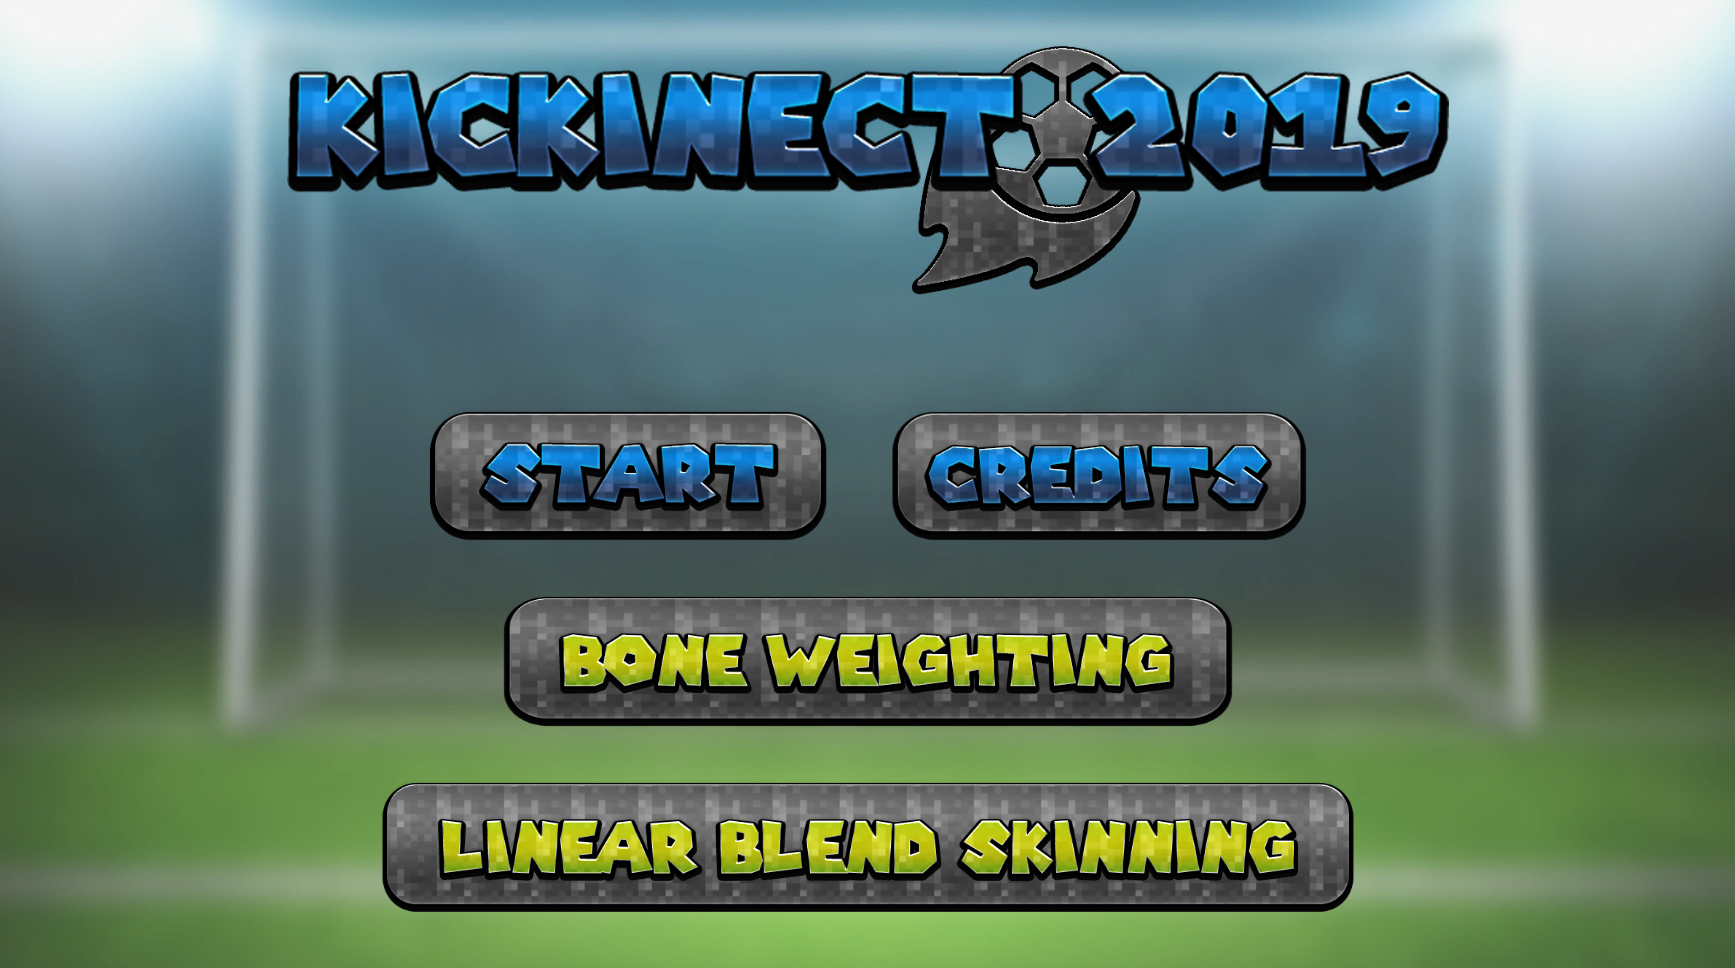
\includegraphics[width=800px]{../Screenshots/intro}
%  \caption{Welcome screen}
%  \label{fig:game}
%\end{figure}

\section{Overview}
A \textit{Microsoft Kinect Sensor} is used to track the player and his movements.
From the raw RGB-D input data a body skeleton is calculated and extracted.
%\image{../Screenshots/weight_colors_cropped.png}{Figure 4: The rest pose mesh and colorful visualized bone weights (left) and the corresponding skeleton bones (right)}{800px}
By using \linearBlendSkinning{} the rest pose mesh is deformed using the kinematic chain transformations $G(\vec{\omega}_j, j)$.
The deformed mesh is assigned to the player game object in a \textit{Unity3D} scene and represents the virtual avatar of the player. \\
The game content now consists of the player controlling the virtual avatar by moving in front of the \kinect{} and shooting the virtual ball into the holes of the goal wall to score as high as possible.\\
%\image{../Screenshots/main/main_goal.png}{Figure 5: The player shooting onto the goal wall}{200px}

%\begin{figure}[h]
%	\centering
%	\includegraphics[width=\linewidth]{overview}
%	\caption{Method overview.}
%	\label{fig:overview}
%\end{figure}

\section{Development process}
We started by settting up the group project in Unity and installing the drivers and the frameworks for the Kinect and its SDK.
From this setup, we created models for the player, the ball and the Torwand and created a scene for it.
Another scene was created for the welcome screen and a simple UI overlay that showed some debugging information as well as an animation for when a goal is hit.

The Kinect SDK already provided a powerful interface and a Unity integration which made it possible to quickly realize our game idea.
This included especially the body movement detection and mapping it to a rigged model. 

At this point, the game was basically ready and we started to replace the SDK with our own implementation of \linearBlendSkinning{} and refine the other parts.
This proved to be more difficult than we anitcipated for various reasons. 

We quickly learned, that performing skeleton detection accurately and efficiently was not an easy task to solve.
The Kineckt SDK uses some rather complex neural networks to predict joint positions from its input streams and thus, we decided to focus on the skinning process only.

We proceeded by pre-recordeding a couple of input videos, since we only had two physical Kinect devices.
This made it possible for everyone to work on the project independently.

\section{Challenges}
  \subsection*{Ball velocity}
  %
  We had to tune the calculation of the velocity with which the ball is accelerated towards the goal wall manually.
  The following aspects had to be taken into account to receive a realistic value:
  \begin{enumerate}
    \setlength{\itemsep}{0pt}
    \item The distance of the player to the goal wall
    \item The overall scaling of the scene
    \item The size of the ball in relation to the player
    \item The amount of hitboxes around the players feet as well as their shape
    \item The angle of the hit and the rapidity of the body movement when swinging the foot
    \item The mass of the ball and the foot
  \end{enumerate}
  The first four aspects can be tuned directly in Unity's physics and model framework by modifying the parameters of the models and rigid bodies.
  For the fifth and sixth aspect, we applied the formula of an elastic collision and received very good results:
  \begin{equation}
    v_{ballshot} = 
    \frac{(2 \cdot m_{\text{ball}} \cdot v_{\text{ball}} + (m_{\text{foot}} - m_{\text{ball}}) \cdot v_{\text{foot}})}{(m_{\text{ball}} + m_{\text{foot}})}
  \end{equation}
  %
  \subsection*{Synchronization}
  %
  The biggest challenge was to synchronize the \kinectSDK{} with \textit{Unity3D}.
  The \kinect{} is recording an RGB-D input stream and through the \kinectSDK{} it provides the joints of the body (25 joints in total) and some orientations.\\
  Even though, ultimately, these values are correct, the joints and rotations do not follow standard character rigging conventions.
  We had to implement a very tough mapping from the received \kinect{} joint data to our rigged character to be able to apply the \linearBlendSkinning{} algorithm presented earlier.\\
  Unfortunately we were not able to integrate correct per bone rotations but could implement the game using some \textit{Unity3D} packages.

\section{Images}
  \image{../Screenshots/intro.png}{Figure 1: Welcome screen with its menu}{400px}
  \image{../Screenshots/weight_colors_cropped.png}{Figure 2: The rest pose mesh and colorful visualized bone weights (left) and the corresponding skeleton bones (right)}{400px}
  \image{../Screenshots/weight_texture.png}{Figure 3: Riged player model (left) with the corresponding skeleton bones (right)}{400px}
  \image{../Screenshots/main/shooting_scene.png}{Figure 4: A player shooting a ball towards the goal wall}{400px}
  \image{../Screenshots/main/main_goal.png}{Figure 5: The player shooting onto the goal wall}{400px}

% references
{\small
	\bibliographystyle{plain}
	\bibliography{project_proposal}
}

\end{document}


